\def\xnode{\node[align=left, draw,thick,circle,black,minimum size=1.0cm,fill=gray!20!white]}
\def\znode{\node[align=left, draw,thick,circle,black,minimum size=1.0cm,fill=white]}

% IMPORTANT: define relative positions of the subpanels here.  Allows easy shuffling.
\def\xa{-6.0}
\def\xb{-2.7}
\def\xc{2.4}

\begin{tikzpicture}[>=triangle 45, triangle/.style = {fill=white, regular polygon, regular polygon sides=3 }]%,transform canvas={scale=0.8}]

% panel A
\node (A) at (\xa+0.2, 0.4) {{\bf A}};

  \xnode (x) at (\xa+2,-2.0) {{\bf $x$}};
 \znode (z) at (\xa+2,0.0) {$z$};
 \node (a0) at (\xa+0.5,0.0) {$\alpha$};
 \node (a) at (\xa+0.5,-2.0) {$\beta$};
  
 \draw[thick,->] (z)--(x);
\draw[thick,->] (a0)--(z);
\draw[thick,->] (a)--(x);
 \node[rectangle,draw=black, thick, rounded corners, fit=(x),inner sep=3.5mm](plate1) {};
 
\node (zx) at (\xa+2,-4.5) {\footnotesize $p(z | x_1,...,x_N) $};
 \node (post) at (\xa+2,-3.0) {};
\draw[thick,dashed,->] (post)--(zx); 
 
% panel B
\node (B) at (\xb+0.3, 0.4) {{\bf B}};
 
 \node[triangle, draw=black, thick,inner sep=3mm](d0) at (\xb + 2.7,-0.4) {}; 
% TRIANGLE PICTURES HERE
 \node (t0) at (\xb + 2.7,-0.4+0.2) {
\includegraphics[width=14mm]{fig/t0.png}};  % include a picture here

 \node[triangle, draw=black, thick,inner sep=3mm](d1) at (\xb + 1.0,-2.3) {}; 
  \node[triangle, draw=black, thick,inner sep=3mm](d2) at (\xb + 2.7,-2.3) {}; 
   \node[triangle, draw=black, thick,inner sep=3mm](d3) at (\xb+4.4,-2.3) {};  
% TRIANGLE PICTURES HERE
 \node (t11) at (\xb + 1.0,-2.3+0.2) {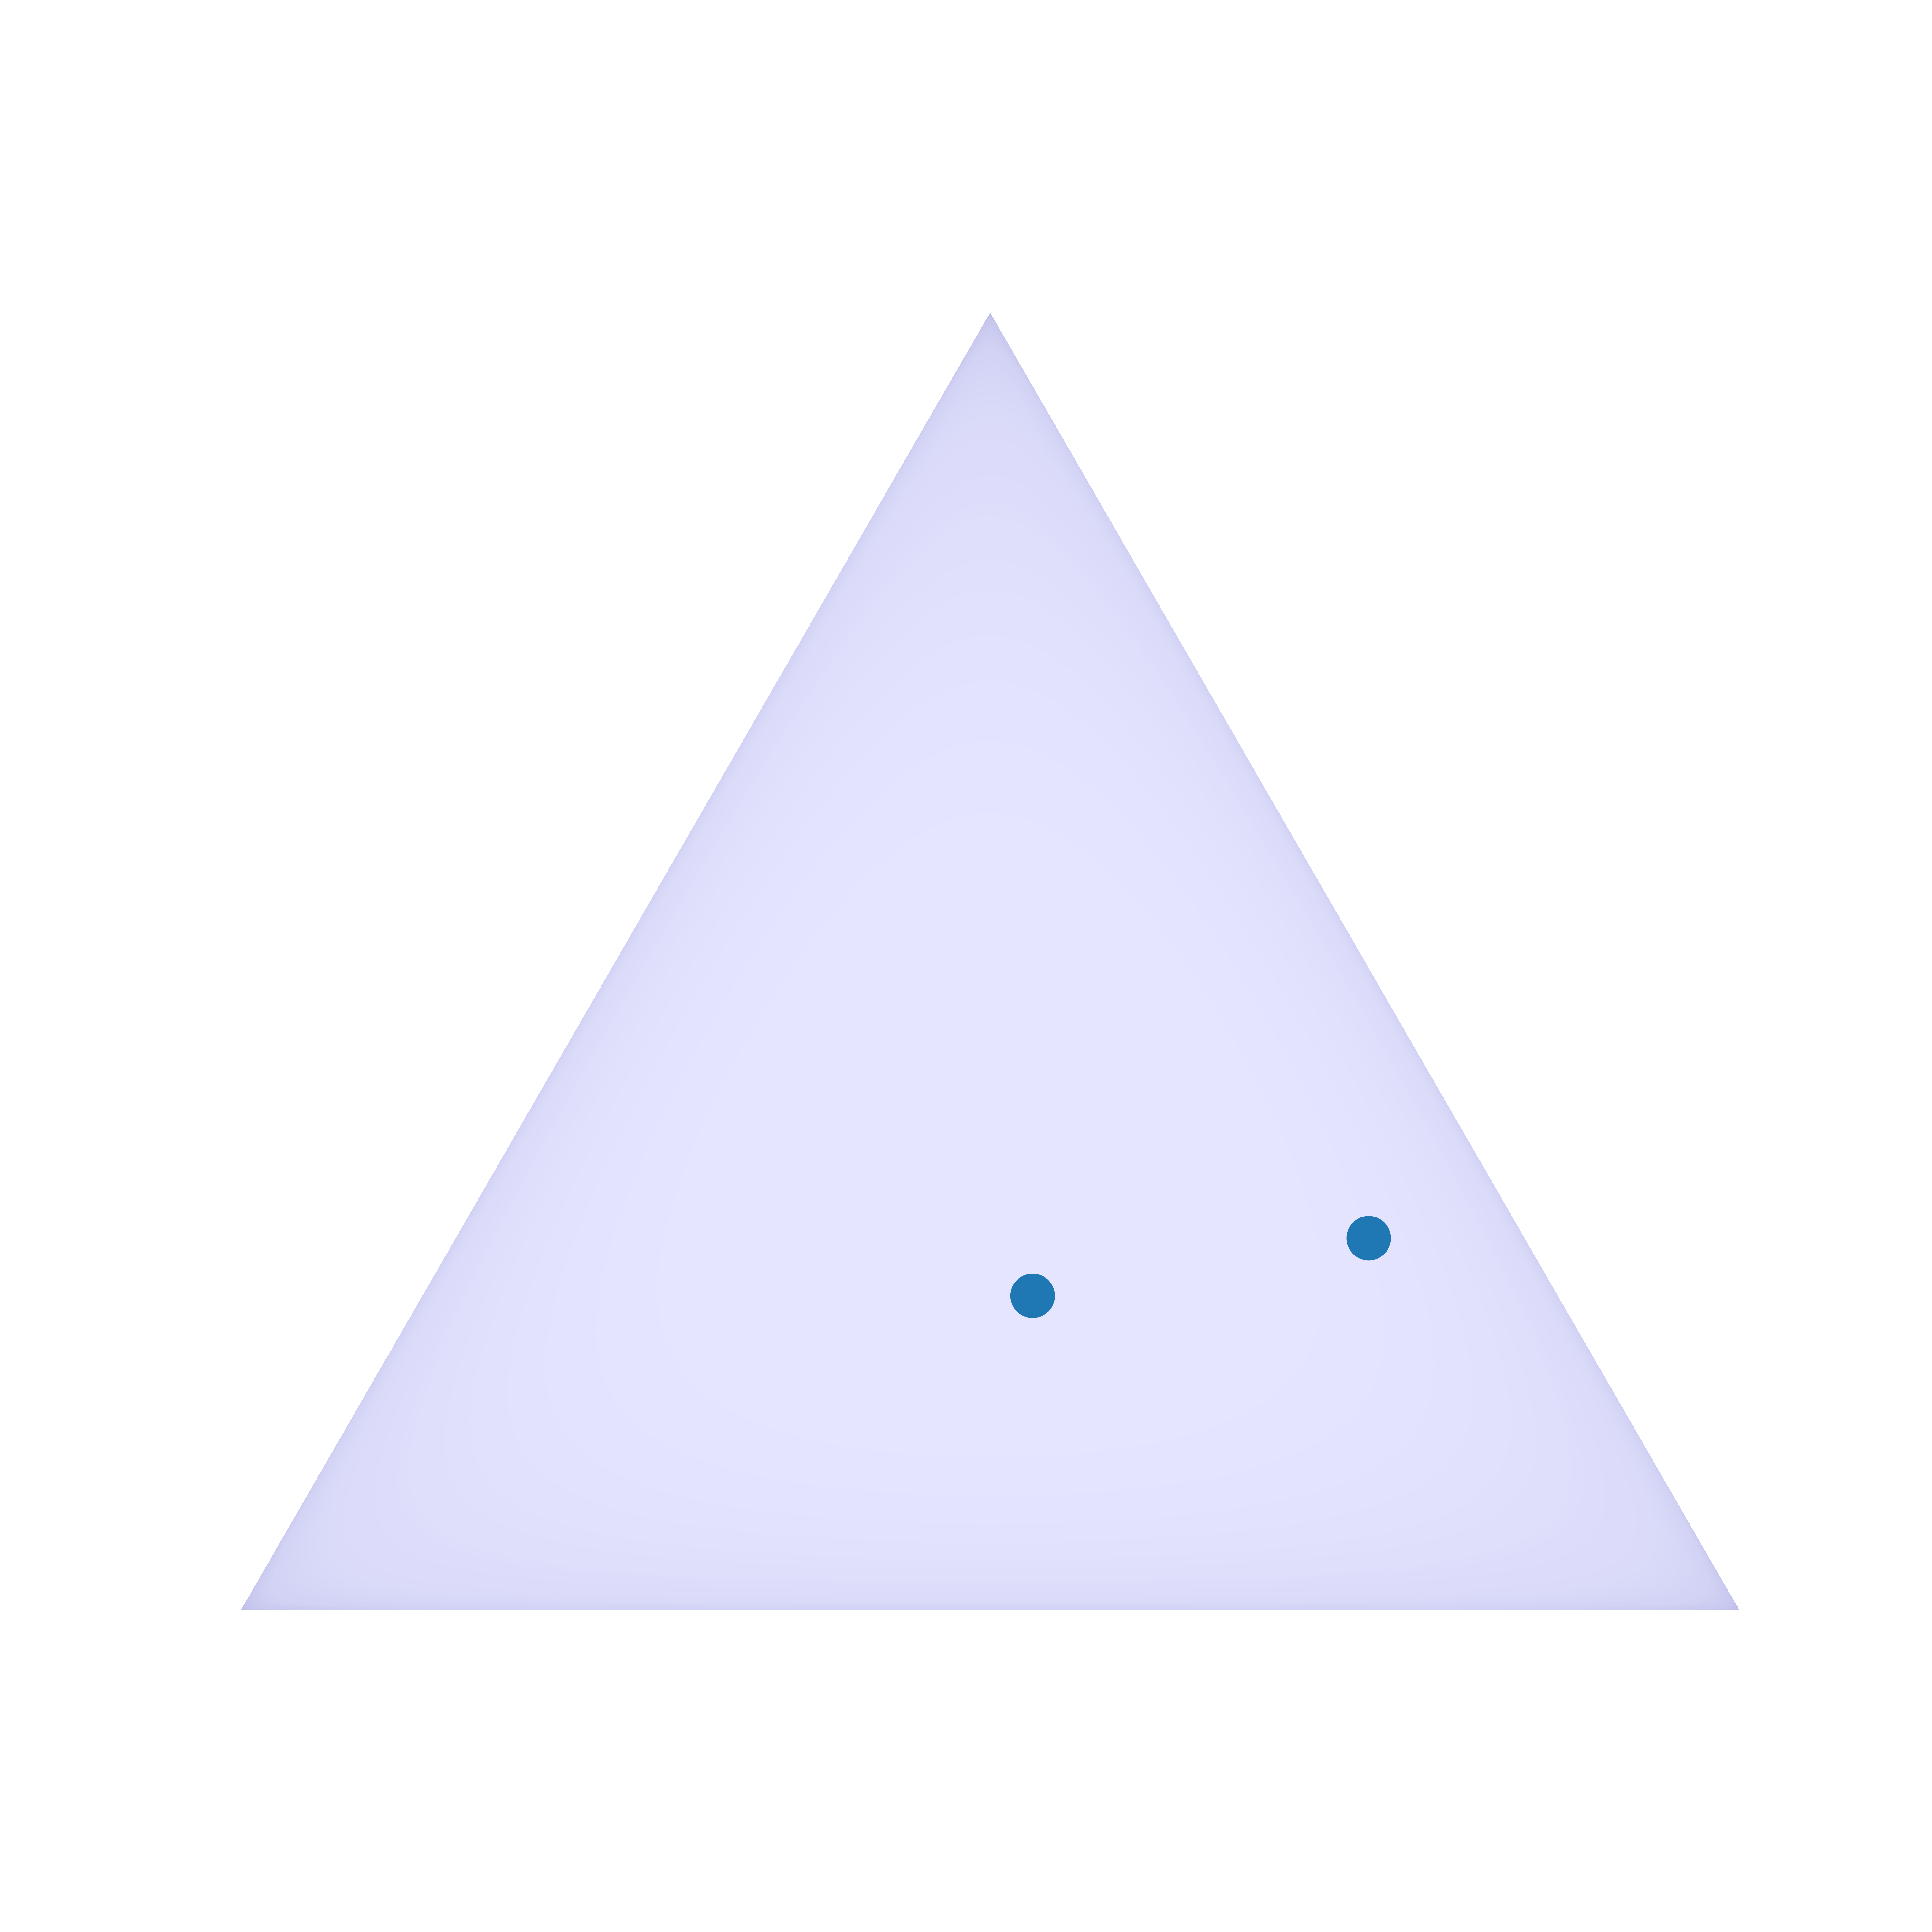
\includegraphics[width=14mm]{fig/t11.png}};  % include a picture here
 \node (t12) at (\xb + 2.7,-2.3+0.2) {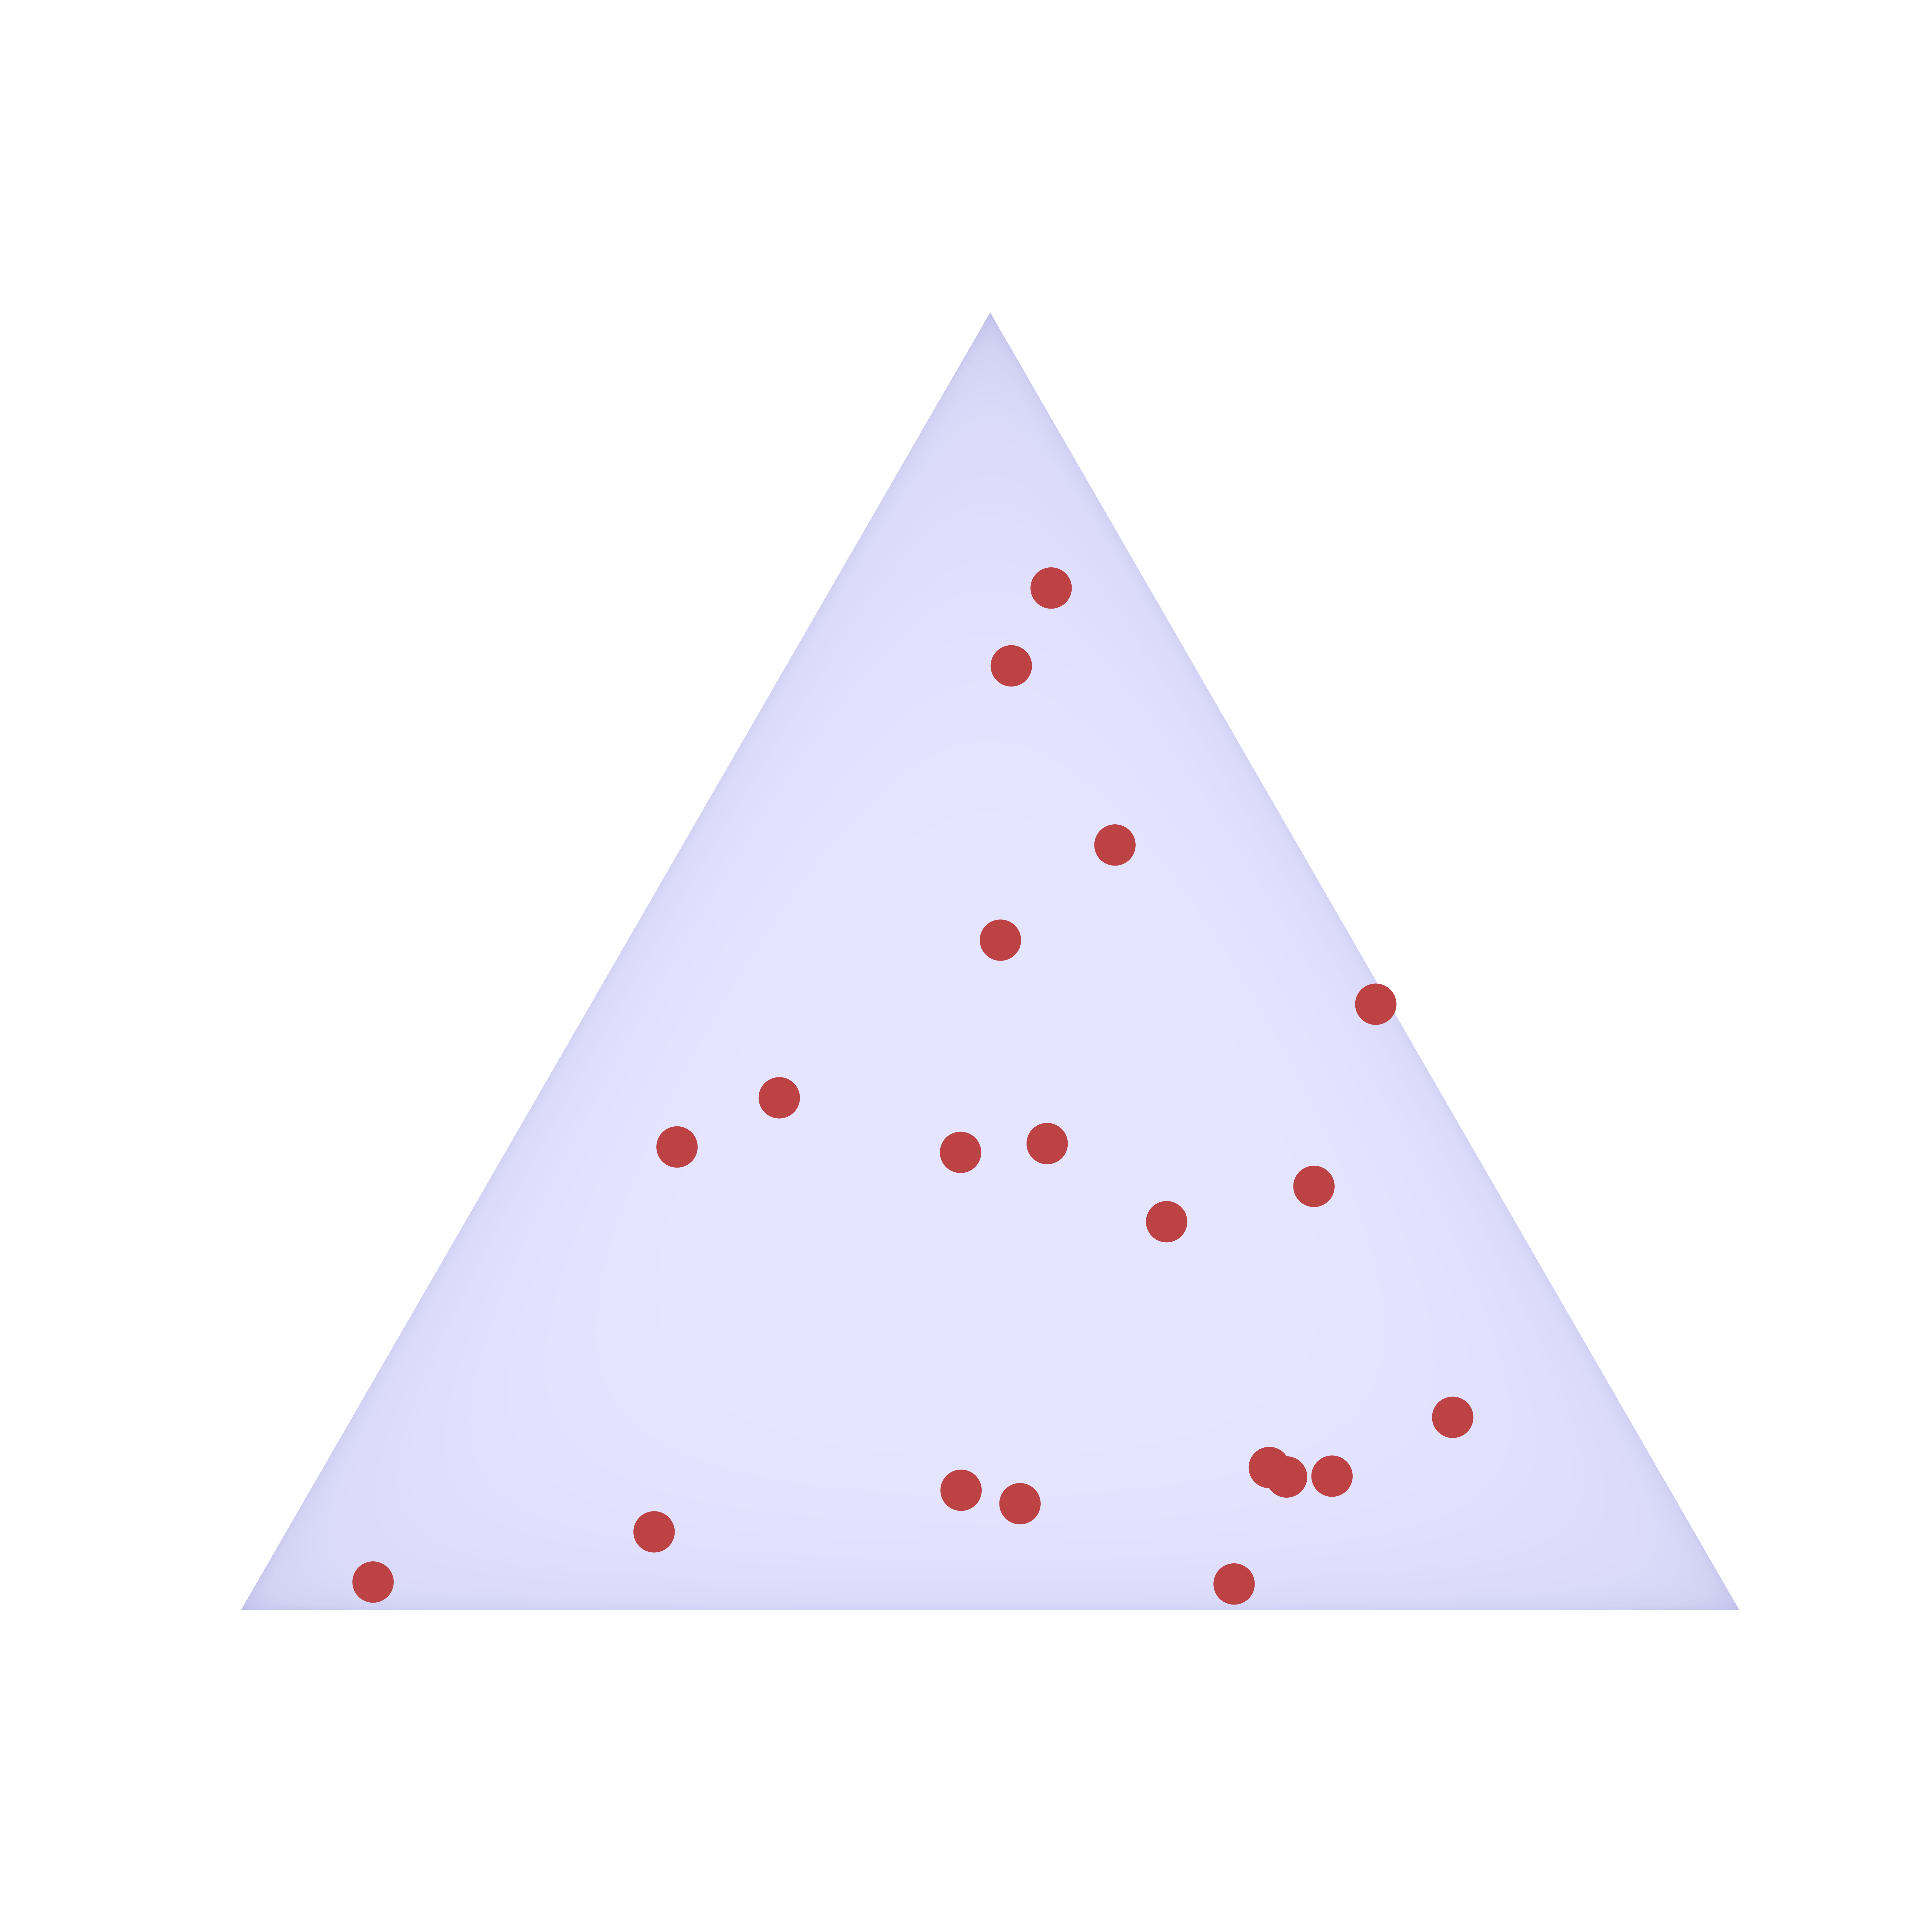
\includegraphics[width=14mm]{fig/t12.png}};  % include a picture here
 \node (t13) at (\xb + 4.4,-2.3+0.2) {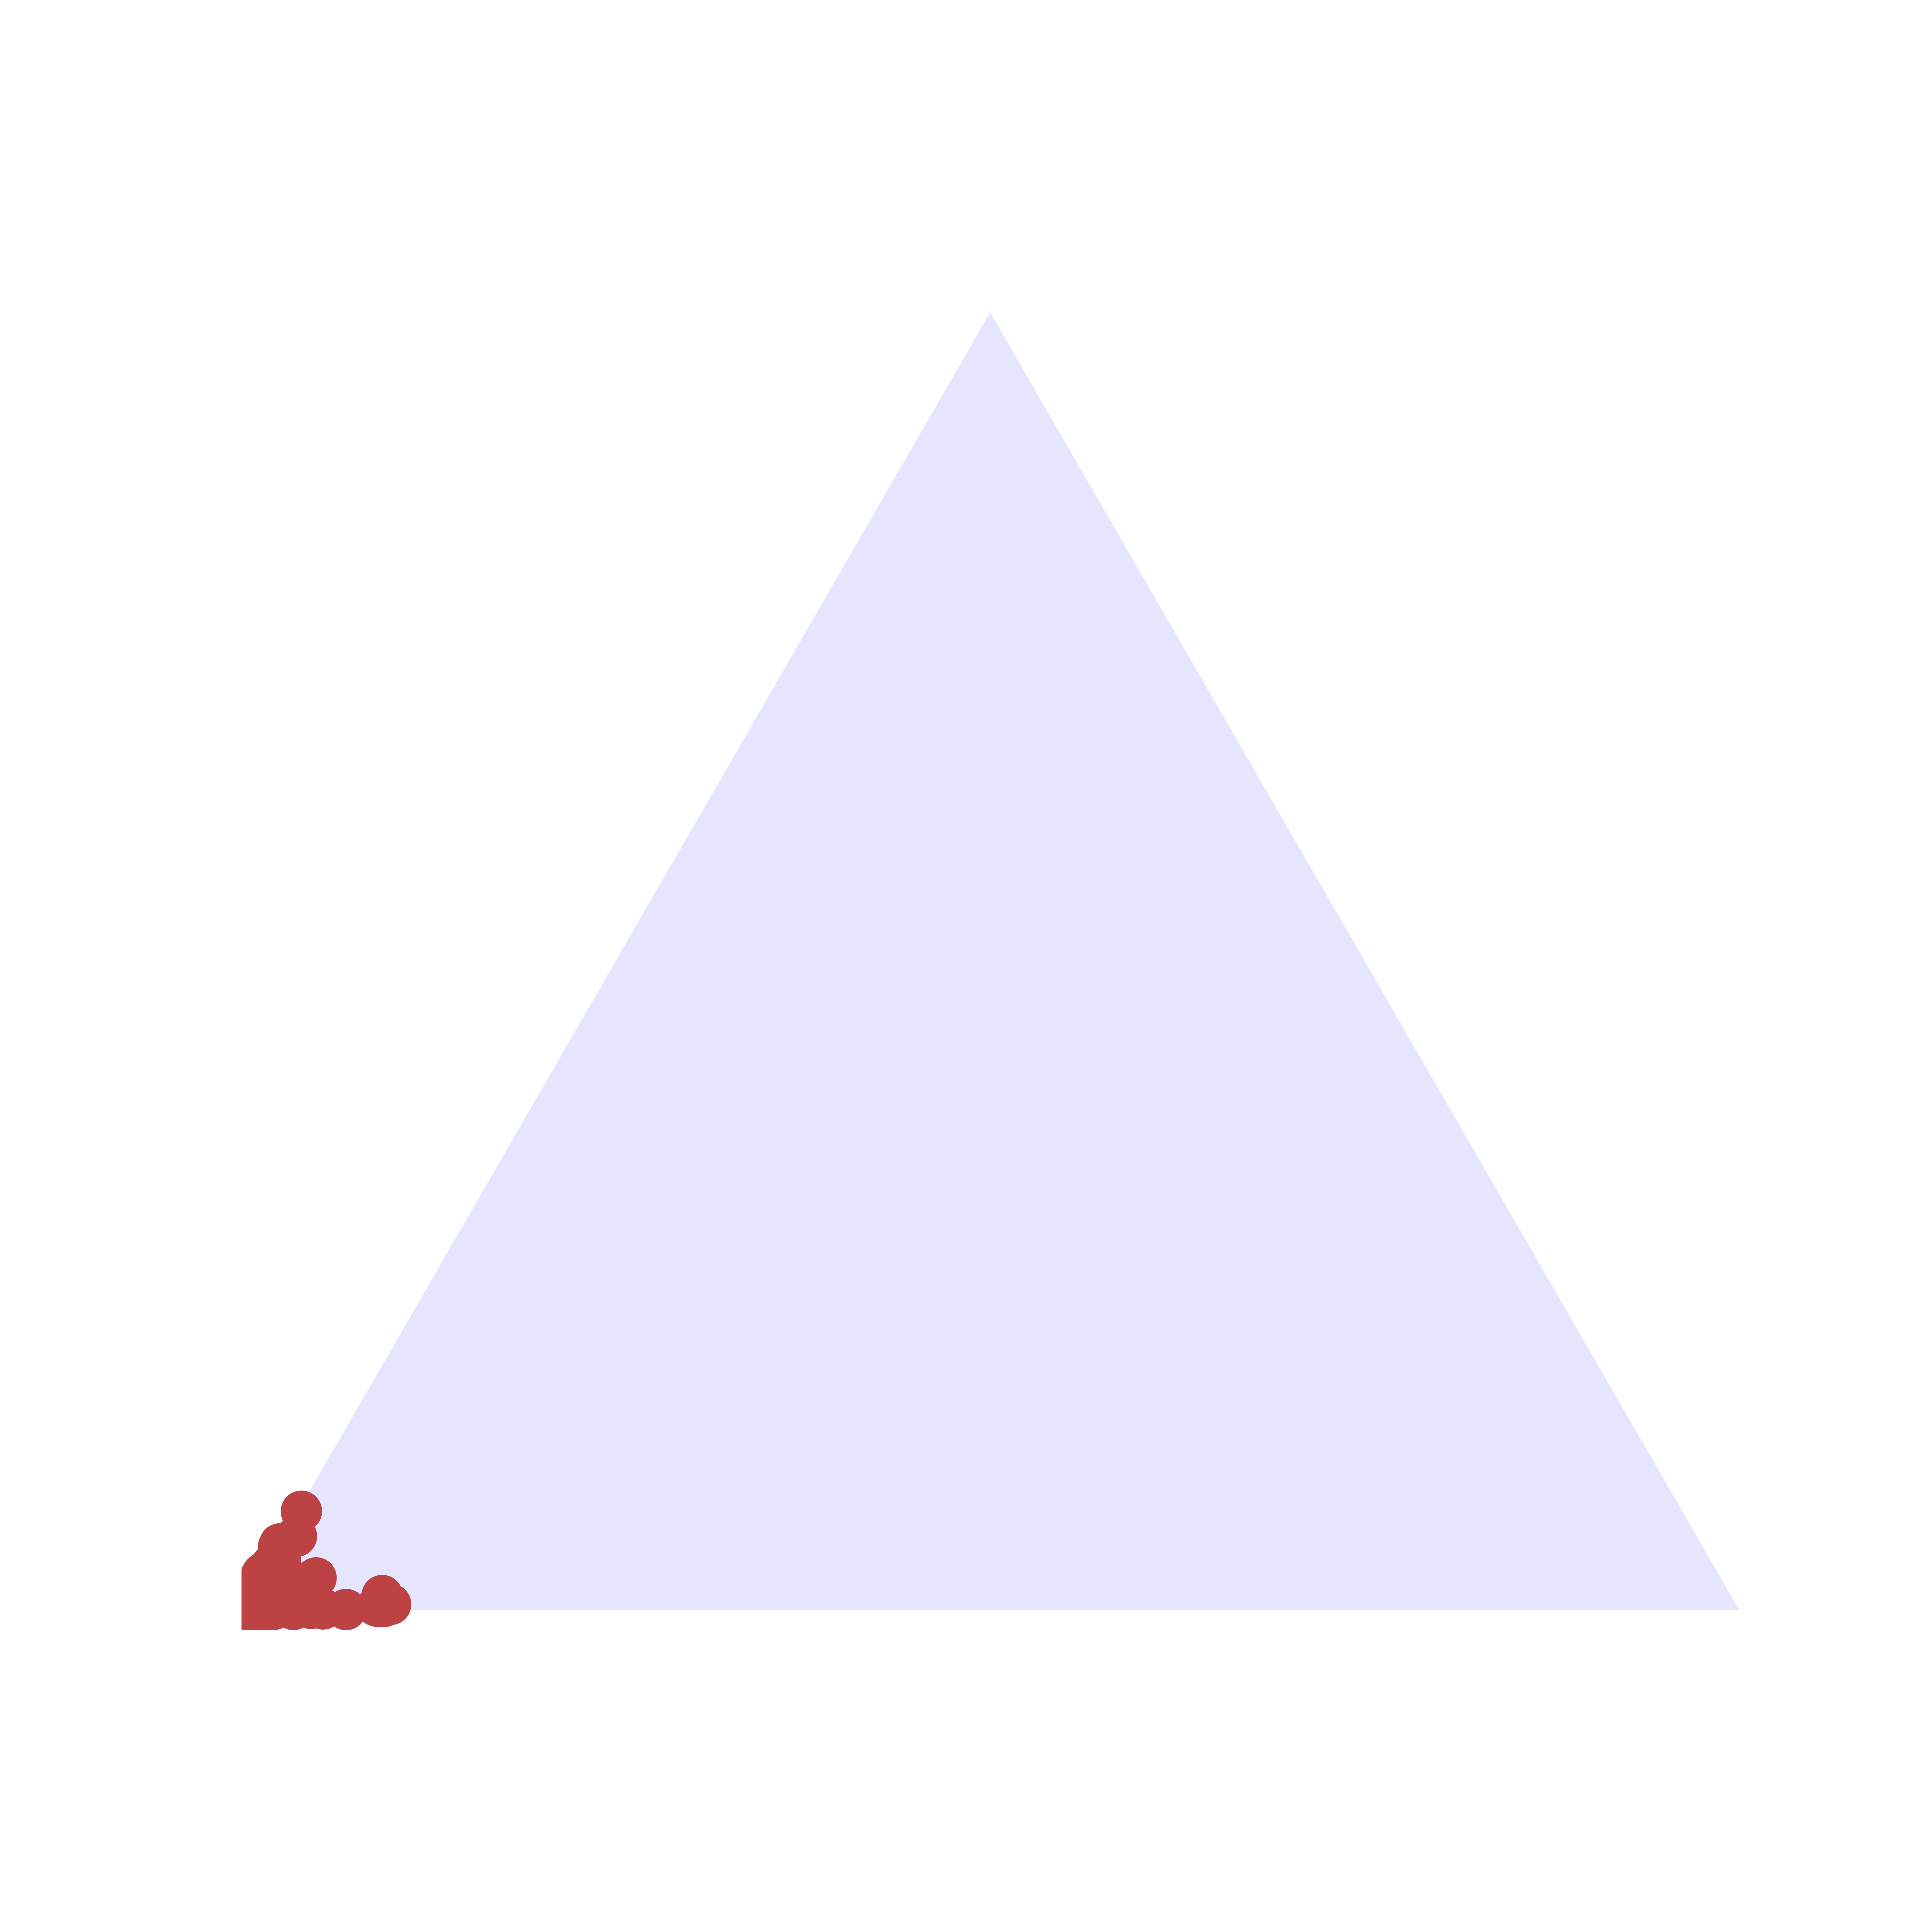
\includegraphics[width=14mm]{fig/t13.png}};  % include a picture here

  \node (dt) at (\xb + 3.5,-2.1){...};

 \node[triangle, draw=black, thick,inner sep=3mm](dp1) at (\xb + 1.0,-4.7) {}; 
  \node[triangle, draw=black, thick,inner sep=3mm](dp2) at (\xb + 2.7,-4.7) {}; 
   \node[triangle, draw=black, thick,inner sep=3mm](dp3) at (\xb + 4.4,-4.7) {};  
% TRIANGLE PICTURES HERE
 \node (t21) at (\xb + 1.0,-4.7+0.2) {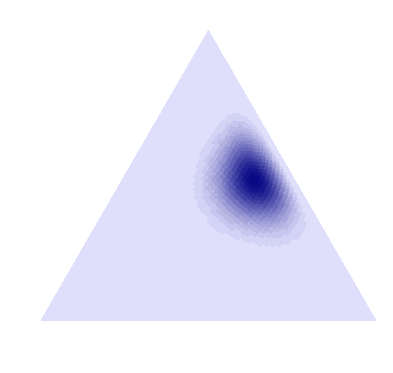
\includegraphics[width=14mm]{fig/t21.png}};  % include a picture here
 \node (t22) at (\xb + 2.7,-4.7+0.2) {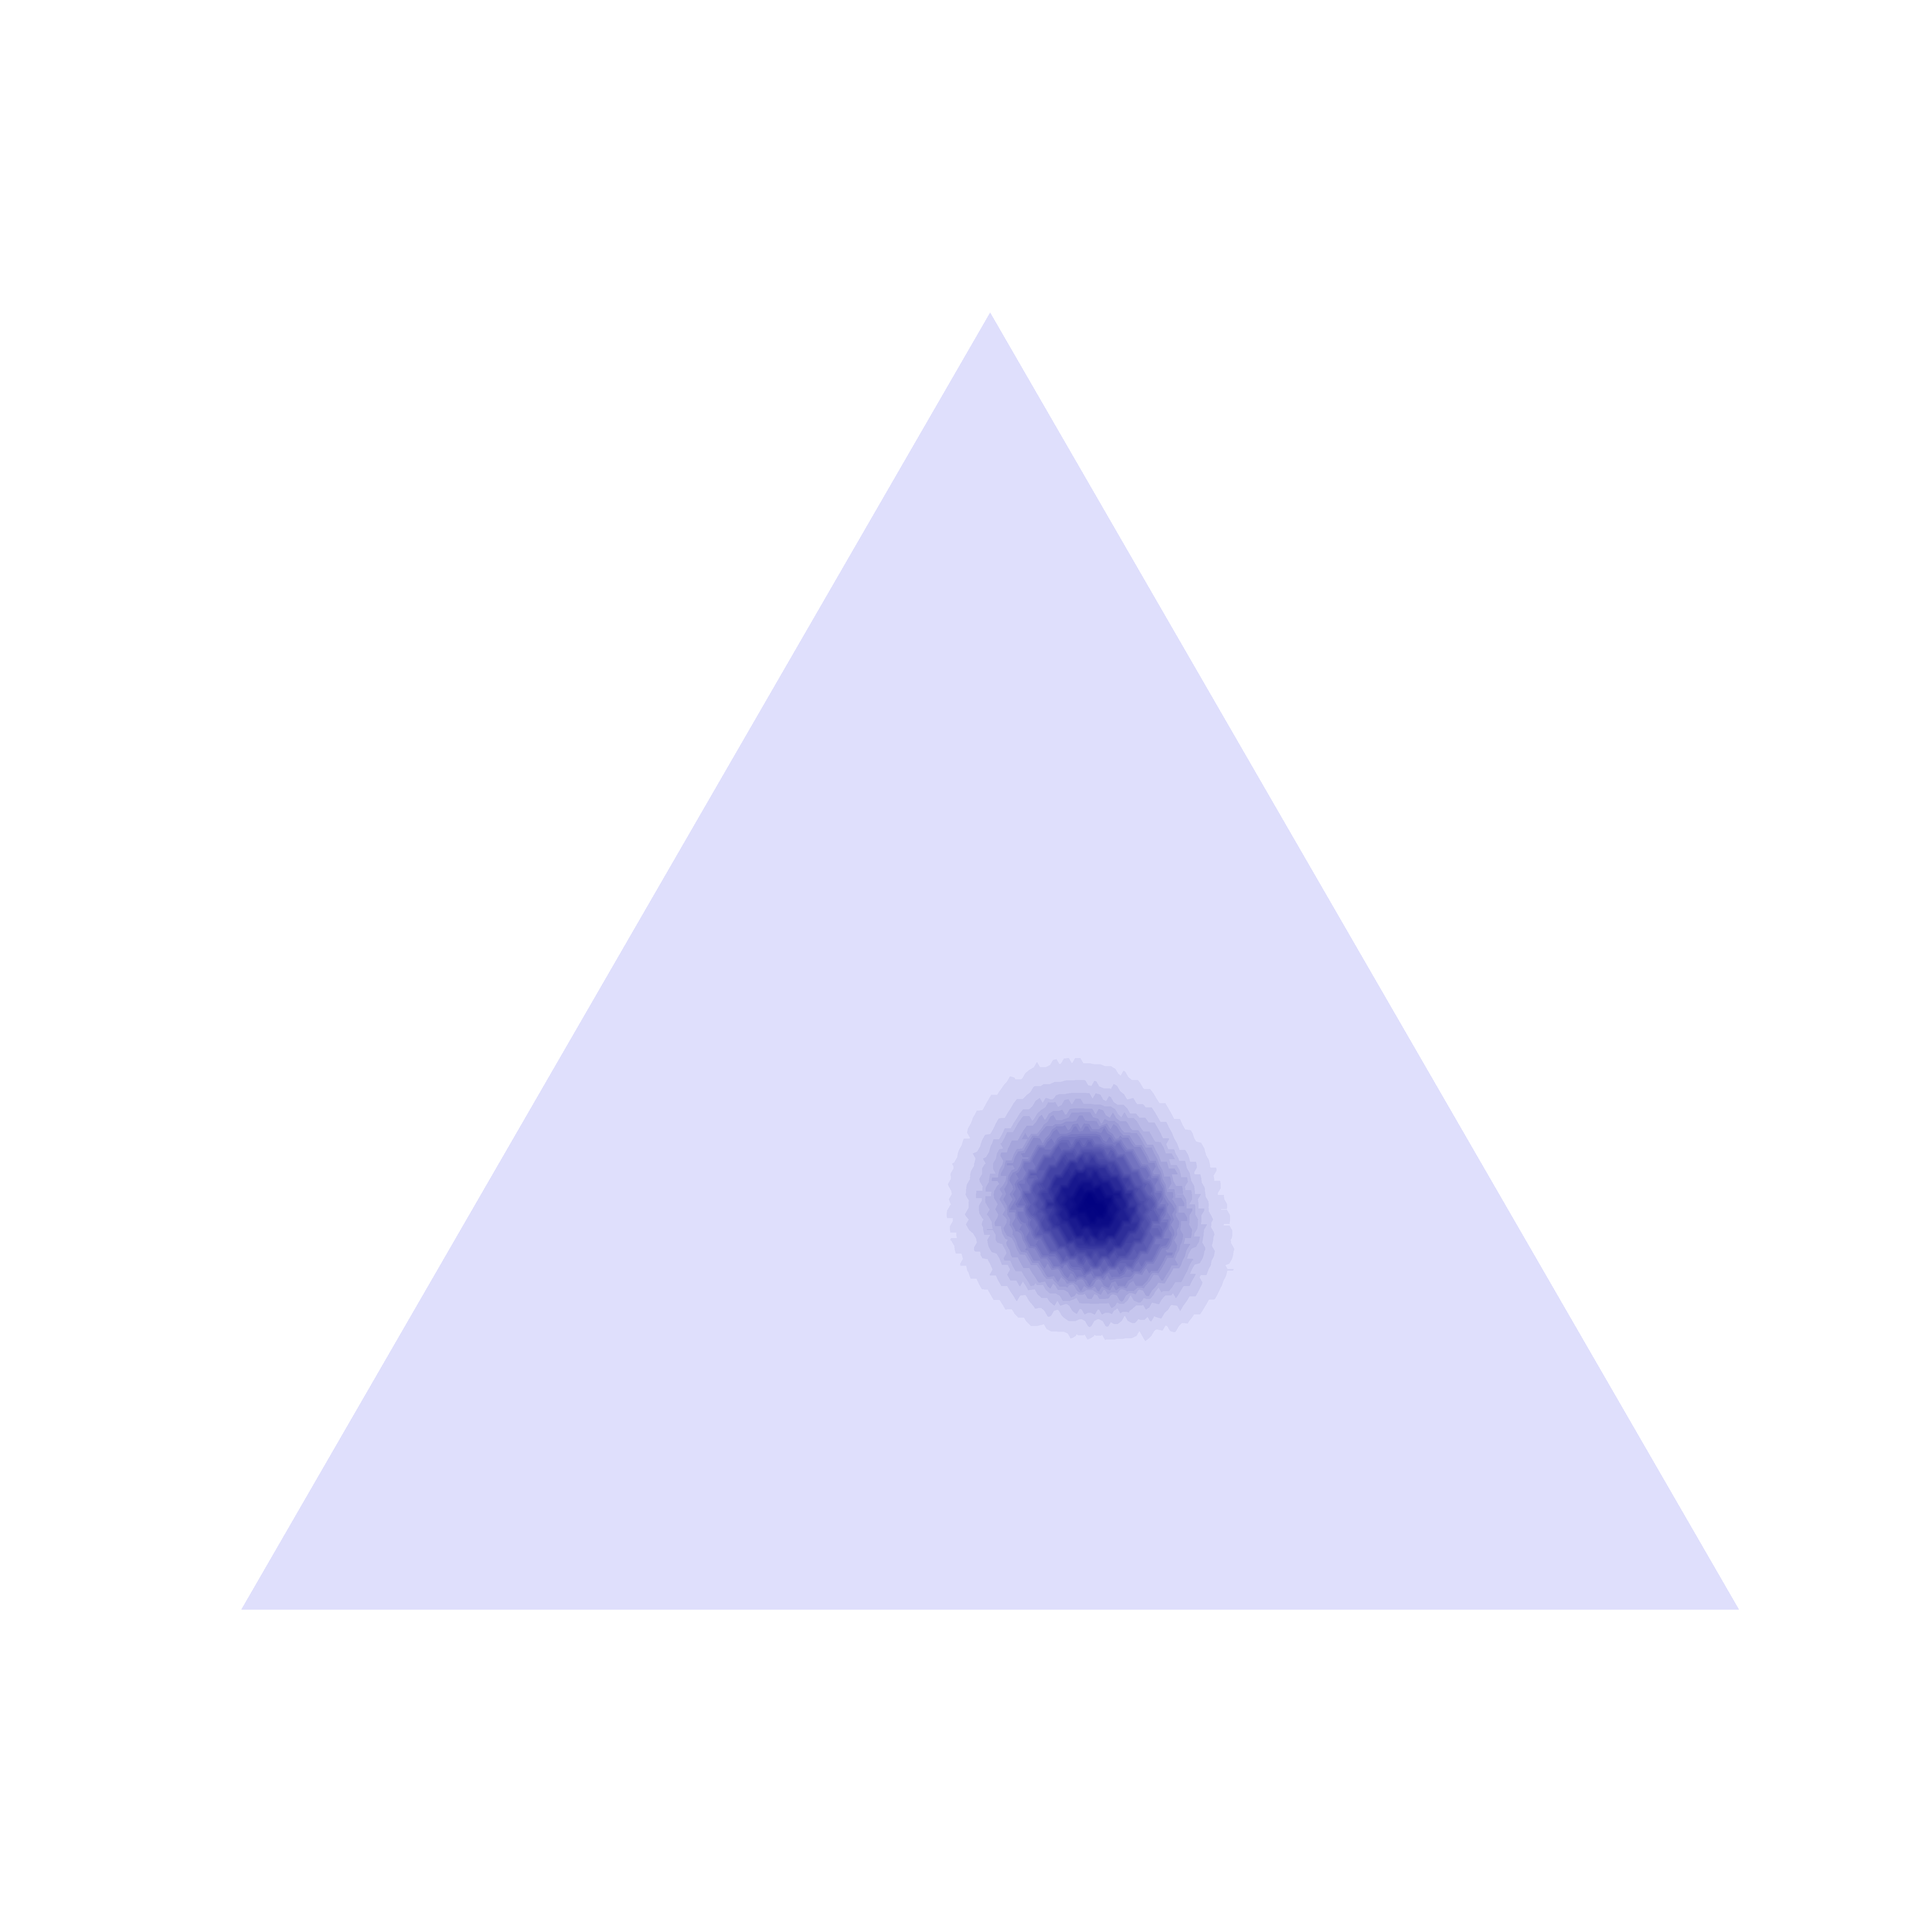
\includegraphics[width=14mm]{fig/t22.png}};  % include a picture here
 \node (t23) at (\xb + 4.4,-4.7+0.2) {
\includegraphics[width=14mm]{fig/t23.png}};  % include a picture here

  \node (dpt) at (\xb + 3.5,-4.3){...};

 \node (p1) at (\xb + 1.0,-2.8) {};
  \node (p2) at (\xb + 2.7,-2.8) {};
   \node (p3) at (\xb + 4.4,-2.8) {};
\draw[thick,dashed,->] (p1)--(dp1); 
\draw[thick,dashed,->] (p2)--(dp2); 
\draw[thick,dashed,->] (p3)--(dp3); 

\draw[thick,->] (d0.south)--(d1.north); 
\draw[thick,->] (d0.south)--(d2.north); 
\draw[thick,->] (d0.south)--(d3.north); 


% panel C
\node (C) at (\xc, 0.4) {{\bf C}};

\node (w) at (\xc+1.5,0.0) {$w \sim \mathcal{N}(0,I)$};

\node (nf1) at (\xc+1.5, -1.1)  {};
\draw[draw=black,thick] (\xc+0.5, -1.2) rectangle ++(2.2,0.2);
\draw[thick,->] (w.south)--(nf1.north);

\node (nf2) at (\xc+1.5, -2.1)  {};
\draw[draw=black,thick] (\xc+0.5, -2.2) rectangle ++(2.2,0.2);
\draw[thick,->] (nf1.south)--(nf2.north);

\node (nf3) at (\xc+1.5, -3.1)  {};
\draw[draw=black,thick] (\xc+0.5, -3.2) rectangle ++(2.2,0.2);
\draw[thick,dotted] (nf2.south)--(nf3.north);

\node (nf4) at (\xc+1.5, -4.4)  {$z \sim q_\phi(z;\eta)$};
\draw[thick,->] (nf3.south)--(nf4.north);

% now the theta of eta network.
\node (eta) at (\xc+5.6, -2.1) {$\eta$};

\node (te1) at (\xc+4.9, -2.1)  {};
\draw[draw=black,thick] (\xc+4.8, -3.2) rectangle ++(0.2,2.2);
\draw[thick,->] (eta)--(te1);

\node (te2) at (\xc+4.3, -2.1)  {};
\draw[draw=black,thick] (\xc+4.2, -3.2) rectangle ++(0.2,2.2);
\draw[thick,->] (te1)--(te2);

\node (te3) at (\xc+3.7, -2.1)  {};
\draw[draw=black,thick] (\xc+3.6, -3.2) rectangle ++(0.2,2.2);
\draw[thick,dotted] (te2)--(te3);


% connect networks
\node (nf1r) at (\xc+2.6, -1.1)  {};
\node (nf2r) at (\xc+2.6, -2.1)  {};
\node (nf3r) at (\xc+2.6, -3.1)  {};
\draw[thick,->] (te3)--(nf1r); 
\draw[thick,->] (te3)--(nf2r); 
\draw[thick,->] (te3)--(nf3r); 

\node (tpe) at (\xc+2.4, -2.5) {$\theta_{\phi} (\eta)$};
\node (phi) at (\xc+4.3, -3.5) {$\phi$};


% \xnode (x) at (-4.0,-2.0) {$x$};
% \znode (z) at (-4.0,0.0) {$z$};
% \node (a) at (-5.0,-2.0) {$\gamma$};
% \node (a0) at (-5.0,0.0) {$\alpha_0$};
%
%  \draw[thick] (x)--(z);
%  \draw[thick] (a0)--(z); 
%  \draw[thick] (a)--(x);
%  
  
%  \gmnode (X) at (0,0) {};
%  \node[align=center] at (X)        {$\sigma\left(\sum_i \!w_{ij}^0 x_{i}^0 \!+\! b_j^1\right)$};
%  \node (X1) at (-3.0,-2.0) {$x_{3}^0$};
%  \node (X2) at (-3.0,0) {$x_{2}^0$};
%  \node (X3) at (-3.0,2.0) {$x_{1}^0$};
%  \node[circle,fill=black] (X4) at (2.5,0) {};
%  \node (X5) at (4.0,-2.0) {...};
%  \node (X6) at (4.0,0.0) {...};
%  \node (X7) at (4.0,2.0) {...};
%  \node (X8) at (1,-2.5) {Neural unit};
%  
%  \draw[thick] (X)--(X1) node[pos=0.8,scale=0.2,label=right:{$w_{3j}^0$}] {};
%  \draw[thick] (X)--(X2) node[pos=0.5,scale=0.2,label=above:{$w_{2j}^0$}] {};
%  \draw[thick] (X)--(X3) node[pos=0.8,scale=0.2,label=right:{$w_{1j}^0$}] {};
%  \draw[thick] (X)--(X4) node[pos=0.5,scale=0.2,label=above:{$x_j^1$}] {};
%  \draw[thick] (X4)--(X5) ;
%  \draw[thick] (X4)--(X6);
%  \draw[thick] (X4)--(X7) node[pos=0.5,scale=0.2,label=right:{}] {};

% \node[obs]                   (x)      {$x$} ; %
%  %\node[latent, above=of T]    (theta)  {$\theta$}; %
%%\node[const, above=of x] (f) {};
%  \node[latent, above=of x]    (z)      {$z$} ; %
%  \node[const, left=of z] (a0) {$\alpha_0$};
%
%\edge {z}{x};
%\edge {a0}{z};
%

%  \plate {plate1} { (x) } {$N$}; %
 
%  % More nodes
%  \factoredge {x}  {z}     {x} ; %
% % Define nodes
%  \node[obs]                               (y) {$y$};
%  \node[latent, above=of y, xshift=-1.2cm] (w) {$\mathbf{w}$};
%  \node[latent, above=of y, xshift=1.2cm]  (x) {$\mathbf{x}$};
%  \node[latent, right=2cm of y]            (t) {$\tau$};
%
%  % Connect the nodes
%  \edge {x,w,t} {y} ; %
%
%  % Plates
%  \plate {yx} {(x)(y)} {$N$} ;
%  \plate {} {(w)(y)(yx.north west)(yx.south west)} {$M$} ;

 
 
  
\end{tikzpicture}
